\documentclass[handout]{beamer}

\usepackage{graphicx}

\usetheme{Pittsburgh}
\usecolortheme{dove}
\usefonttheme{serif}

\title{Formulação e Implementação da Amostragem de Importância Múltipla em um Path Tracer}
\author{Gustavo Silveira Frehse}
\institute[UFPR]{
  Departamento de Informática\\
  Universidade Federal do Paraná
}
\date{2026}

\AtBeginSection[]{
  \begin{frame}
    \centering
    \Huge\insertsection
  \end{frame}
}

\begin{document}

\frame{\titlepage}

\begin{frame}

\frametitle{toc}
\tableofcontents
\end{frame}

% ========================================================================

\section{Introdução}

\begin{frame}
\frametitle{Introdução}

\begin{itemize}
  \item<1-> A síntese de imagens fotorrealísticas tem como objetivo gerar
    imagens dada uma descrição de uma cena.
  \item<2-> O \emph{Path Tracing} é uma das técnicas que mais se aproxima da
    descrição física da luz, permitindo efeitos realistas.
  \item<3-> É bastante custosa, tornando a procura de técnicas de otimização
    uma grande área de pesquisa.
\end{itemize}
\end{frame}

% ========================================================================

\begin{frame}
\frametitle{Objetivo}

\begin{itemize}
  \item<1-> Modificar um Ray Tracer básico para utilizar a técnica de
    Amostragem de Importância Múltipla e analisar os resultados.
    \begin{itemize}
      \item<2-> Para isso, escolher as a técnicas de amostragem e formular os
        pesos da técnica. 
      \item<3-> Mostrar as modificações feitas. 
    \end{itemize}
\end{itemize}
\end{frame}

% ========================================================================

\section{Equação da renderização}


% ------------------

\subsection{Intuição}

\begin{frame}
\frametitle{Intuição}

\begin{enumerate}
  \item<1-> Abstraímos o problema para cada pixel. 
  \item<2-> Cada pixel tem uma direção associada.
  \item<3-> Luz chegou dessa direção.
  \item<4-> Continuamos nessa direção até achar um ponto na geometria.
    \begin{itemize}
      \item<5-> É possível que batemos direto em uma fonte de luz. 
    \end{itemize}
  \item<6-> Para cada direção no hemisfério, voltamos ao terceiro passo,
  ponderando com o ângulo e uma distribuição de peso.
    \begin{itemize}
      \item<7-> Como temos infinitas direções, não conseguimos obter soluções
      exatas em geral. 
      \item<8-> Para a modelagem, porém, podemos usar a maquinaria do cálculo.
    \end{itemize}
\end{enumerate}

\end{frame}

% ------------------

\subsection{A equação}

\begin{frame}
\frametitle{A equação}

\[
\begin{aligned}
    \uncover<1->{L(x, \omega_o) ={}&} \uncover<2->{L_e(x, \omega_o)} \\
     \uncover<3->{&+\int_{\omega_i \in \mathcal{H}}} \uncover<4->{L(\gamma(x, \omega_i),
    -\omega_i)} \uncover<5->{f_s(x, \omega_i \rightarrow \omega_o)} \uncover<6->{| \cos\theta |}
    \uncover<7->{d\sigma_x(\omega_i)}
\end{aligned}
\]

\end{frame}

% ========================================================================

\section{Monte Carlo}

% ------------------

\subsection{Monte Carlo simples}

\begin{frame}
\frametitle{Monte Carlo simples}

\begin{itemize}
  \item<1-> Para uma integral
  \[
    I = \int_{x \in D} f(x) dx
  \]
  \item<2-> Podemos criar um estimador de Monte Carlo
  \[
    I_N = \frac{1}{N} \cdot \sum_{i=1}^N \frac{f(X_i)}{p(X_i)}
  \]
\end{itemize}

\end{frame}

% ------------------

\subsection{Amostragem de importância}

\begin{frame}
\frametitle{Amostragem de importância}
  \[
    I_N = \frac{1}{N} \cdot \sum_{i=1}^N \frac{f(X_i)}{p(X_i)}
  \]

\begin{itemize}
  \item<2-> Podemos escolher $p$! (Cada $p$ corresponde à uma técnica de amostragem)
  \item<3-> Quanto mais perto da forma de $f$, menor a variância do estimador,
  e menos amostras precisamos.
  \item<4-> Objetivo: achar um $p$ bom.
  \item<5-> Problema: nem sempre é possível.
    \begin{itemize}
      \item<6-> Para algumas situações certos $p$ são melhores, em outras
        outros $p$ levam vantagem.
    \end{itemize}
\end{itemize}

\end{frame}

\begin{frame}
  \frametitle{Ilustração}
  \[
    {\setbeamercovered{transparent}\uncover<1-1>{\begin{aligned}
      L(x, \omega_o) ={}& L_e(x, \omega_o) \\ &+\int_{\omega_i \in
      \mathcal{H}} L(\gamma(x, \omega_i), -\omega_i) f_s(x, \omega_i
      \rightarrow \omega_o) | \cos\theta | d\sigma_x(\omega_i)
    \end{aligned}}}
  \]
  \[
    \uncover<2->{\begin{aligned}
      f ={}& L(\gamma(x, \omega_i), -\omega_i) f_s(x, \omega_i
      \rightarrow \omega_o) | \cos\theta | 
    \end{aligned}}
  \]
  \centering
  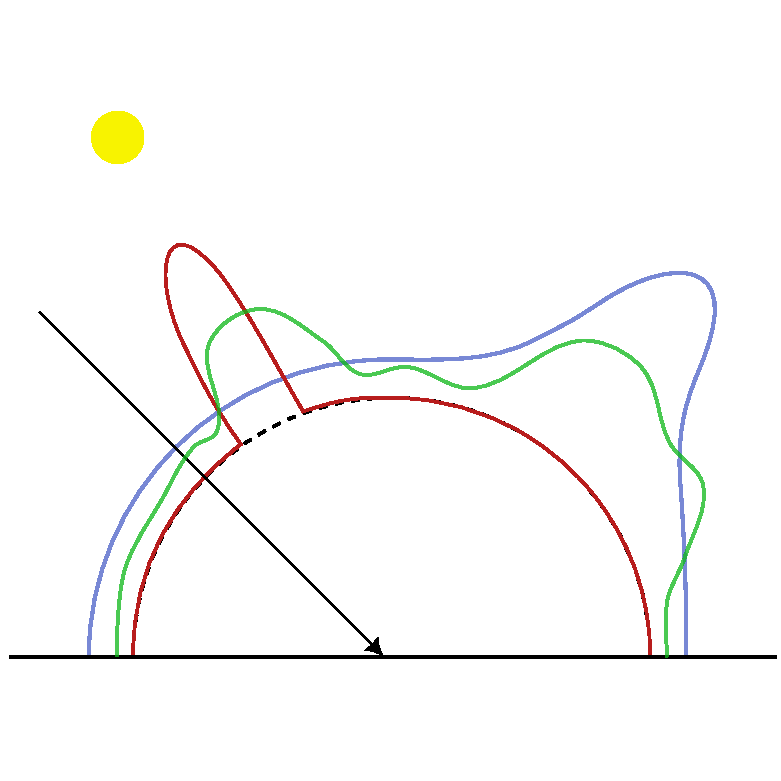
\includegraphics[width=0.6\textwidth]{f.pdf}
\end{frame}

% ========================================================================

\section{Amostragem de Importância Múltipla}

\begin{frame}
\frametitle{Amostragem de Importância Múltipla}

  \begin{itemize}
    \item<1-> A Amostragem de Importância Múltipla permite combinar múltiplas
      amostras, colocando pesos nas amostras.
    \item<2-> Assim, estratégias melhores para uma direção terão maiores pesos
      naquela direção.
    \item<3-> Podemos escrever o estimador como
      \begin{equation*}
        I = \sum_{i=1}^n \frac{1}{n_i} \sum_{j=1}^{n_i} w_i(X_{i,j})
          \frac{f(X_{i,j})}{p_i(X_{i,j})}
      \end{equation*}
  \end{itemize}
\end{frame}
% ========================================================================

\section{Formulação de Pesos}

\begin{frame}
\frametitle{Equação de Caminhos}

  \begin{itemize}
    \item<1-> Podemos escrever a Equação da Renderização como um soma das integrais
      de cada caminho de tamanho $k$ (desenrolamos a recursão):
      \[
        \begin{aligned}
        \sum_{k=0}^\infty \int_{\bar{x} \in \mathcal{P}_k}
        &\, L_e(x_k, \omega_{o,k}) \\
        &\times \left(
        \prod_{m=2}^{k-1}
        f(x_m, \omega_{i,m} \rightarrow \omega_{o,m})
        |\cos\theta_m|
        \right) \\
        &\times d\sigma_{x_1}(\omega_{i,1})
        \cdots
        d\sigma_{x_k}(\omega_{i,k}).
        \end{aligned}
      \]
    \item<2-> Assim podemos amostrar cada caminho de uma vez, e usar a
      Amostragem de Importância Múltipla em caminhos de diferentes tamanhos ao
      mesmo tempo.
  \end{itemize}
\end{frame}

\begin{frame}
\frametitle{Formulação}
  \begin{itemize}
    \item<1-> Fazemos um caminho base, e a cada vértice desse caminho
      amostramos a fonte de luz para possivelmente fechar um caminho completo.
    \item<2-> Temos duas formas de formar um caminho específico,
      \begin{itemize}
        \item<3-> Com cada vértice sendo amostrado pelo BRDF e o último sendo pela fonte de luz,
        \item<4-> e com todos os vértices sendo amostrados pelo BRDF, inclusive a fonte de luz. 
      \end{itemize}
    \item<5-> Assim podemos fazer a Amostragem de Importância Múltipla com essas duas técnicas.
  \end{itemize}
\end{frame}

\begin{frame}
\frametitle{Implementação}
  \begin{itemize}
    \item<1-> Fazemos um \emph{loop} para gerar o caminho base.
    \item<2-> Em cada iteração, amostramos a luz. Se não houver obstruções adicionamos a contribuição com o devido peso.
    \item<3-> Amostramos um novo ponto com BRDF. Caso esse ponto seja na luz, adicionamos a contribuição com o devido peso.
    \item<4-> Fazemos uma Roleta Russa para ver se continuamos esse caminho base.
  \end{itemize}
\end{frame}
% ========================================================================

\section{Resultados}
\begin{frame}
\frametitle{Métodos de avaliação}
  \begin{itemize}
    \item<1->São feitas duas análises:
    \begin{itemize}
      \item<2->As imagens resultantes com e sem cada uma das técnicas de
        amostragens, assim como as imagens de variância produzidas por elas.
      \item<3->Os resultados da mesma cena em três tipos de
        iluminação diferentes: luz pequena, luz grande, e ambas.
    \end{itemize}
  \item<4->Para todos os resultados renderizamos imagens em tamanho 1000x1000,
    com 64 estimações por pixel.
  \end{itemize}
\end{frame}

\begin{frame}
\frametitle{Resultados com contribuições diferentes}

  \begin{figure}
    \begin{columns}[T,onlytextwidth]
    \column{0.32\textwidth}
    \centering
    
\includegraphics[width=\linewidth]{complete64spp1000x1000onlybrdf/output.png}
    {\scriptsize Apenas BRDF}
    \vspace{0.5em}
    
\includegraphics[width=\linewidth]{complete64spp1000x1000onlybrdf/variance.png}
    {\scriptsize Variância apenas BRDF}
    \column{0.32\textwidth}
    \centering
    
\includegraphics[width=\linewidth]{complete64spp1000x1000onlynee/output.png}
    {\scriptsize Apenas Fontes de Luz}
    \vspace{0.5em}
    
\includegraphics[width=\linewidth]{complete64spp1000x1000onlynee/variance.png}
    {\scriptsize Variância apenas Fontes de Luz}
    \column{0.32\textwidth}
    \centering
    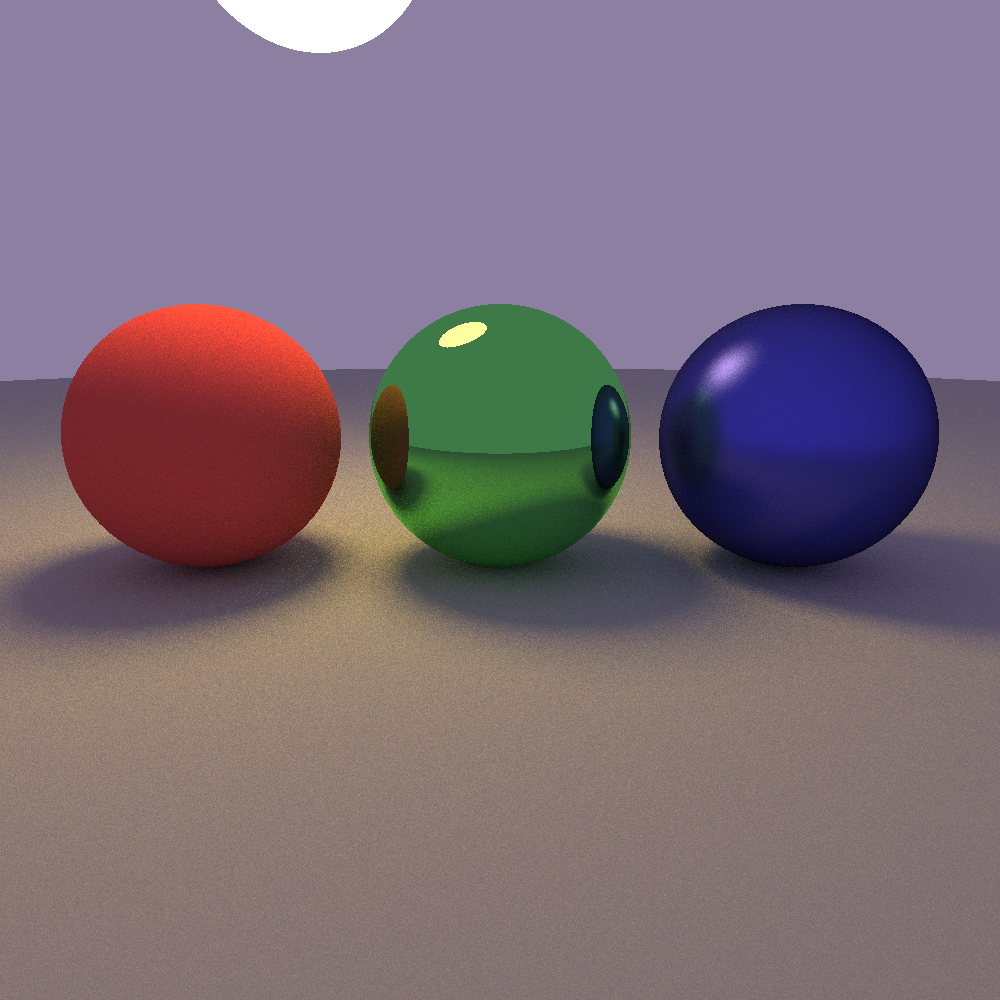
\includegraphics[width=\linewidth]{complete64spp1000x1000/output.png}
    {\scriptsize BRDF + Fontes de Luz}
    \vspace{0.5em}
    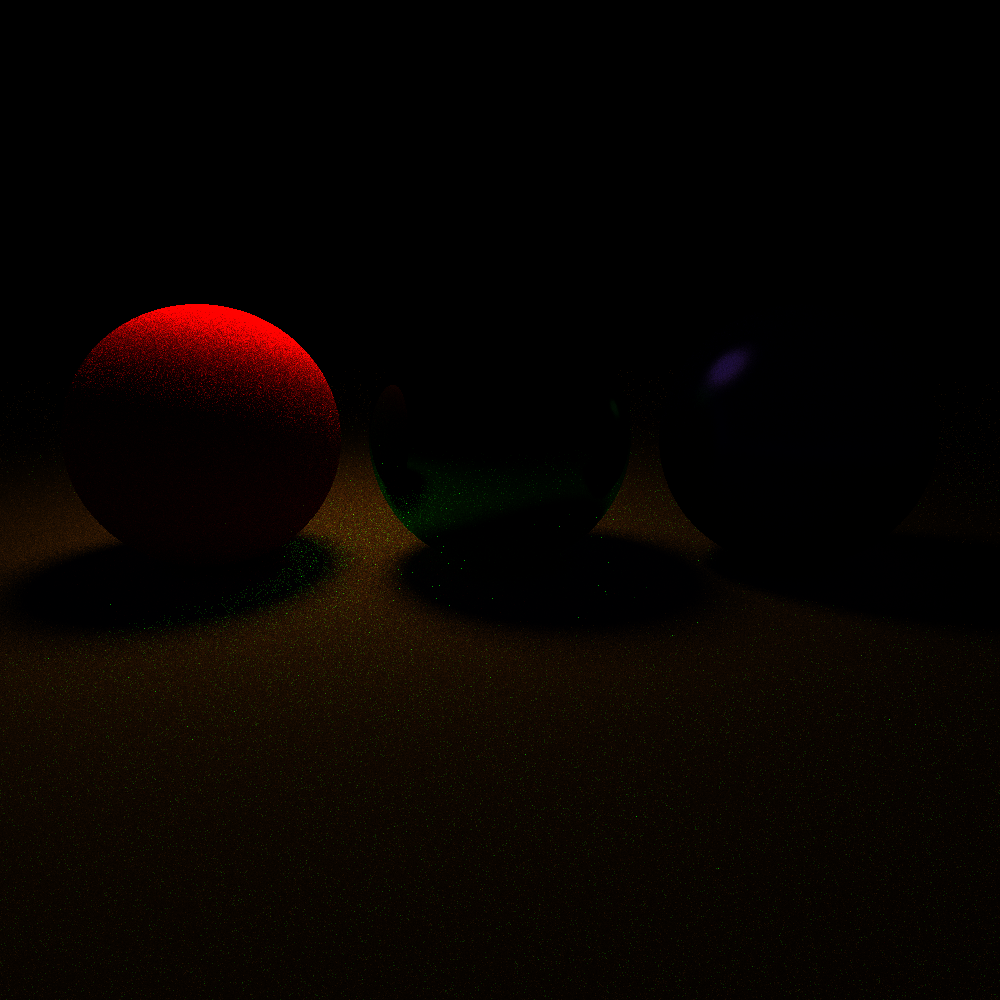
\includegraphics[width=\linewidth]{complete64spp1000x1000/variance.png}
    {\scriptsize Variância BRDF + Fontes de Luz}
    \end{columns}
  \end{figure}
\end{frame}

\begin{frame}
\frametitle{Resultados com cenas diferentes}
\begin{figure}
  \begin{columns}[T,onlytextwidth]

  \column{0.32\textwidth}
  \centering
  
\includegraphics[width=\linewidth]{smalllight64spp1000x1000/output.png}

  {\scriptsize Fonte de luz pequena}

  \vspace{0.5em}

  
\includegraphics[width=\linewidth]{smalllight64spp1000x1000/mis_viz.png}

  \column{0.32\textwidth}
  \centering
  
\includegraphics[width=\linewidth]{skylight64spp1000x1000/output.png}

  {\scriptsize Fonte de luz grande}

  \vspace{0.5em}

  
\includegraphics[width=\linewidth]{skylight64spp1000x1000/mis_viz.png}

  \column{0.32\textwidth}
  \centering
  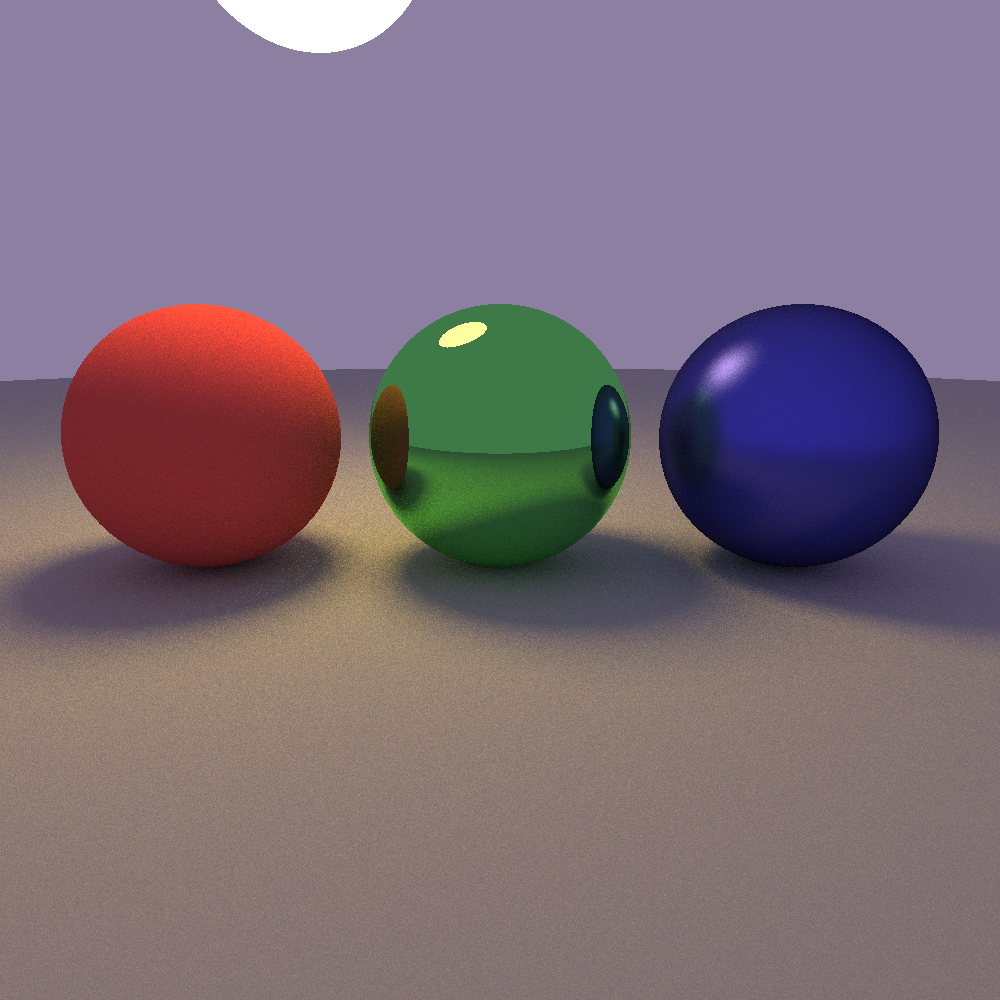
\includegraphics[width=\linewidth]{complete64spp1000x1000/output.png}

  {\scriptsize Duas fontes de luz}

  \vspace{0.5em}

  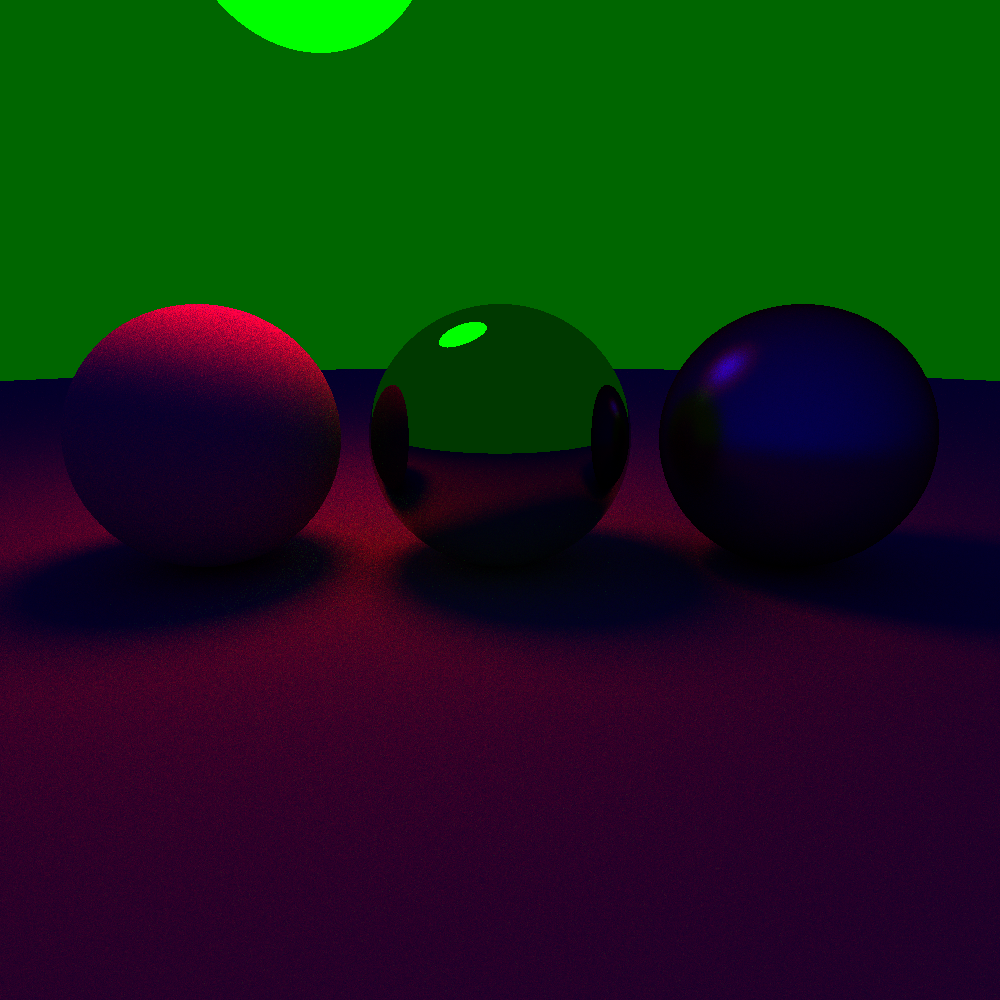
\includegraphics[width=\linewidth]{complete64spp1000x1000/mis_viz.png}

  \end{columns}
\end{figure}

\end{frame}
% ========================================================================

\section{Conclusão}

\begin{frame}
\frametitle{Conclusão}

  \begin{itemize}
    \item<1-> A Amostragem de Importância Múltipla permite a combinação de
      técnicas de amostragem, ponderando cada uma dinamicamente, aproveitando
      os benefícios individuais de cada uma. 
    \item<2-> Com isso conseguimos obter resultados significantemente melhores
      em cenas diversas do que utilizando apenas uma técnica de cada vez.
    \item<3-> Como base de técnicas mais avançadas
  \end{itemize}

\end{frame}
\end{document}
